\documentclass{slides}
\title{Shooting auto flow}
\author{Natan Jurca}
\date{March 2026}

\usepackage{tikz}
\usepackage[top=1cm, bottom=1cm, right=1cm, left=1cm]{geometry}
\usetikzlibrary{shapes.geometric, arrows}
\usetikzlibrary{positioning}

\tikzstyle{startstop} = [rectangle, rounded corners, minimum width=3cm, minimum height=1cm,text centered, draw=black, fill=red!30]
\tikzstyle{io} = [trapezium, trapezium left angle=70, trapezium right angle=110, minimum width=3cm, minimum height=1cm, text centered, draw=black, fill=blue!20]
\tikzstyle{process} = [rectangle, minimum width=3cm, minimum height=1cm, text centered, draw=black, fill=orange!20]
\tikzstyle{decision} = [diamond, aspect=4, minimum width=3cm, minimum height=1cm, text centered, draw=black, fill=green!20]
\tikzstyle{arrow} = [thick,->,>=latex]

\begin{document}
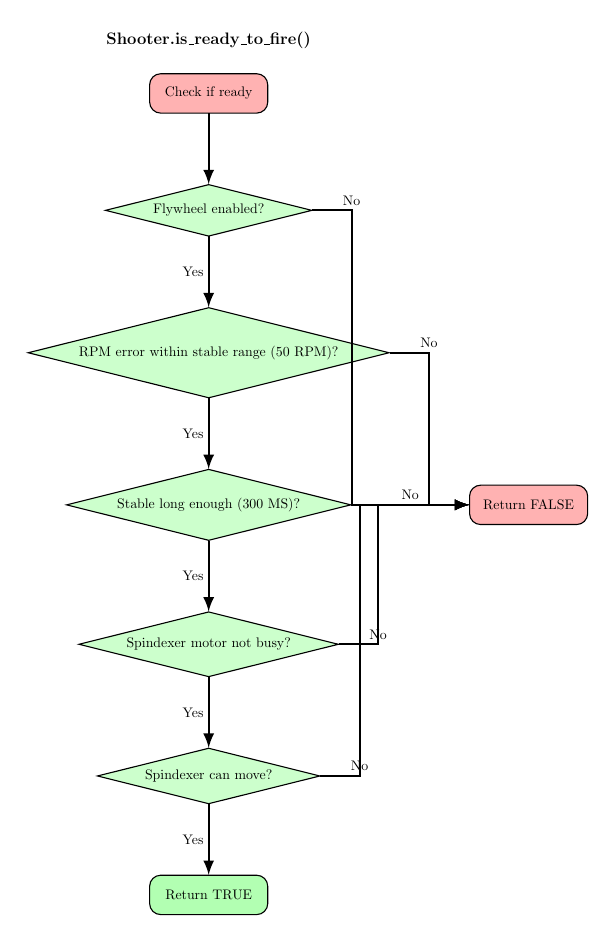
\begin{tikzpicture}[node distance=1.2cm]

% ===== MAIN FLOW (left side) =====
%\begin{scope}[scale=0.85, transform shape]

% Start
%\node (start) [startstop] {Start};

% Init hardware
%\node (init) [process, below=of start] {Initialize Hardware};

% Drive to obelisk
%\node (drive1) [process, below=of init] {Drive to Obelisk Position};

% Wait decision
%\node (wait) [decision, below=1.8cm of drive1] {Pattern seen OR 5s at obelisk OR 10s elapsed in opmode?};

% No - keep waiting (moved to the left)
%\node (waiting) [process, left=2.5cm of wait] {Keep Looking};

% Drive to shooting
%\node (drive2) [process, below=1.8cm of wait] {Drive to Shooting Position};

% Survey check
%\node (survey) [decision, below=1.8cm of drive2] {Spindexer survey complete?};

% Get next color
%\node (nextcolor) [process, below=1.8cm of survey] {Determine next ball color from pattern};

% Ball in shooter?
%\node (ballinshooter) [decision, below=1.8cm of nextcolor] {Ball in shooter?};

% Rotate spindexer
%\node (rotate) [process, right=3cm of ballinshooter, text width=3.5cm] {Rotate spindexer to correct color (or other if unavailable)};

% Ready to fire?
%\node (ready) [decision, below=1.8cm of ballinshooter] {Shooter ready AND 1s since last shot?};

% Fire
%\node (fire) [process, below=1.8cm of ready] {Fire ball, increment score};

% Exit check
%\node (exitcheck) [decision, below=1.8cm of fire] {3 balls scored OR 24s elapsed?};

% Drive to end
%\node (drive3) [process, below=1.8cm of exitcheck] {Stop shooter, set holding pattern, drive to end};

% End
%\node (end) [startstop, below=of drive3] {End};

% Main flow arrows
%\draw [arrow] (start) -- (init);
%\draw [arrow] (init) -- (drive1);
%\draw [arrow] (drive1) -- (wait);
%\draw [arrow] (wait) -- node[anchor=south] {No} (waiting);
%\draw [arrow] (waiting) |- ([yshift=0.5cm]wait.north) -- (wait);
%\draw [arrow] (wait) -- node[anchor=east] {Yes} (drive2);
%\draw [arrow] (drive2) -- (survey);
%\draw [arrow] (survey.west) -- ++(-1.5,0) node[anchor=south east] {No} |- ([yshift=0.5cm]survey.north) -- (survey.north);
%\draw [arrow] (survey) -- node[anchor=east] {Yes} (nextcolor);
%\draw [arrow] (nextcolor) -- (ballinshooter);
%\draw [arrow] (ballinshooter) -- node[anchor=south] {No} (rotate);
%\draw [arrow] (rotate.south) -- ++(0,-0.5) -| (ready.east);
%\draw [arrow] (ballinshooter) -- node[anchor=east] {Yes} (ready);
%\draw [arrow] (ready.west) -- ++(-1.5,0) node[anchor=south east] {No} |- ([yshift=0.5cm]survey.north) -- (survey.north);
%\draw [arrow] (ready) -- node[anchor=east] {Yes} (fire);
%\draw [arrow] (fire) -- (exitcheck);
%\draw [arrow] (exitcheck.west) -- ++(-2,0) node[anchor=south east] {No} |- ([yshift=0.5cm]survey.north) -- (survey.north);
%\draw [arrow] (exitcheck) -- node[anchor=east] {Yes} (drive3);
%\draw [arrow] (drive3) -- (end);

%\end{scope}

% ===== SHOOTER READY FLOW (right side) =====
\begin{scope}[scale=0.5, transform shape]

% Title
\node (title2) [font=\bfseries\large] {Shooter.is\_ready\_to\_fire()};

% Start
\node (s2start) [startstop, below=0.5cm of title2] {Check if ready};

% Flywheel enabled?
\node (flywheelen) [decision, below=1.8cm of s2start] {Flywheel enabled?};

% RPM in range?
    \node (rpmrange) [decision, below=1.8cm of flywheelen] {RPM error within stable range (50 RPM)?};

% Stable long enough?
    \node (stabletime) [decision, below=1.8cm of rpmrange] {Stable long enough (300 MS)?};

% Spindexer motor not busy?
\node (motorfree) [decision, below=1.8cm of stabletime] {Spindexer motor not busy?};

% Spindexer can move?
\node (canmove) [decision, below=1.8cm of motorfree] {Spindexer can move?};

% Return true
\node (rettrue) [startstop, below=1.8cm of canmove, fill=green!30] {Return TRUE};

% Return false
\node (retfalse) [startstop, right=3cm of stabletime, fill=red!30] {Return FALSE};

% Shooter ready arrows
\draw [arrow] (s2start) -- (flywheelen);
\draw [arrow] (flywheelen) -- node[anchor=east] {Yes} (rpmrange);
\draw [arrow] (flywheelen.east) -- ++(1,0) node[anchor=south] {No} |- (retfalse.west);
\draw [arrow] (rpmrange) -- node[anchor=east] {Yes} (stabletime);
\draw [arrow] (rpmrange.east) -- ++(1,0) node[anchor=south] {No} |- (retfalse.west);
\draw [arrow] (stabletime) -- node[anchor=east] {Yes} (motorfree);
\draw [arrow] (stabletime) -- node[anchor=south] {No} (retfalse);
\draw [arrow] (motorfree) -- node[anchor=east] {Yes} (canmove);
\draw [arrow] (motorfree.east) -- ++(1,0) node[anchor=south] {No} |- (retfalse.west);
\draw [arrow] (canmove) -- node[anchor=east] {Yes} (rettrue);
\draw [arrow] (canmove.east) -- ++(1,0) node[anchor=south] {No} |- (retfalse.west);

\end{scope}

\end{tikzpicture}%
\end{document}
